% !TEX program = xelatex
\documentclass[UTF8,a4paper,11pt,fontset=windows]{ctexart}
\usepackage[a4paper,top=2.15cm,bottom=2.15cm,left=2.35cm,right=2.35cm]{geometry}
\usepackage{fontspec}
\setmainfont{Times New Roman}
\setCJKmainfont[BoldFont=Microsoft YaHei]{SimSun}
\setCJKsansfont{Microsoft YaHei}
\usepackage{amsmath,amssymb,bm,booktabs,tabularx,array,longtable}
\usepackage{graphicx,float,caption}
\usepackage{siunitx}
\usepackage{enumitem,setspace,fancyhdr}
\usepackage[hidelinks]{hyperref}
\usepackage{bookmark}
\graphicspath{{assets/}}
\sisetup{detect-all,per-mode=symbol}
\setstretch{1.20}
\emergencystretch=2em
\setlength{\parindent}{2em}
\setlength{\parskip}{0.16em}
\setlength{\tabcolsep}{4pt}
\renewcommand{\arraystretch}{1.18}
\captionsetup{font=small,labelsep=quad}
\setlist[itemize]{leftmargin=2em,itemsep=0.15em,topsep=0.3em}
\newcolumntype{Y}{>{\raggedright\arraybackslash}X}
\newcommand{\code}[1]{\texttt{#1}}
\pagestyle{fancy}
\fancyhf{}
\fancyhead[L]{\small 无人机编队智能避障项目技术报告}
\fancyhead[R]{\small V1.1.1 · 2026-09-24}
\fancyfoot[C]{\thepage}
\setlength{\headheight}{15pt}
\renewcommand{\headrulewidth}{0.35pt}

\begin{document}
\hypersetup{pageanchor=false}
\begin{titlepage}
\thispagestyle{empty}
\centering
\vspace*{2.8cm}
{\heiti\zihao{0} 无人机编队智能避障项目技术报告\par}
\vspace{0.9cm}
{\songti\zihao{2} 现行配置、三参数环境扫描与性能边界\par}
\vspace{2.0cm}
\rule{0.75\textwidth}{0.5pt}\par
\vspace{1.0cm}
\begin{tabular}{@{}rl@{}}
软件版本： & V1.1.1，本地 F 盘工作区快照 \\
现行限速： & \SI{3.0}{m/s} \\
主实验： & 125 个参数组合，每组 seed 1--200 \\
主实验规模： & 25\,000 次计划仿真 \\
实验平台： & MATLAB R2024a，二维静态圆障碍仿真 \\
\end{tabular}
\vfill
{\zihao{4} 2026 年 9 月 24 日\par}
\end{titlepage}
\hypersetup{pageanchor=true}

\pagenumbering{Roman}
\begin{abstract}
本项目以一架长机和四架僚机组成的领航--跟随编队为对象，在二维静态圆障碍环境中结合膨胀栅格规划、改进人工势场（APF）、Actor--Critic 自适应动态规划（ADP）及预测式避碰，实现目标到达和终端归队（以固定 V 形为基准，参考点保留避障修正）。现行源码的最大速度为 \SI{3}{m/s}，长机规划净空为 \SI{4.2}{m}；随机场景的整队可行性筛选采用更大的有效净空 \SI{5.6}{m}。

本次在障碍物数量 4--20 个、航线两侧散布半宽 10--30 m、障碍物最小边缘间距 1--5 m 的 125 个组合上，各运行 seed 1--200，共完成 25\,000 次计划试验。结果为 24\,783 次成功、1 次碰撞、7 次超时、209 次场景生成失败，无程序执行异常。对已生成并完成判定的 24\,791 张地图，飞行成功率为 99.9677\%；将生成失败纳入分母的整体成功比例为 99.132\%。在固定散布半宽 \SI{20}{m}、最小边缘间距 \SI{3}{m} 时，障碍物从 4 个增加到 20 个，成功样本平均完成时间从 \SI{32.37}{s} 增至 \SI{41.57}{s}，长机平均路径系数从 1.036 增至 1.309。

扫描中的飞行成功率接近上限，难以可靠区分多数参数组合的安全性能；高密度、小散布宽度和大间距的组合则暴露出场景生成约束。本报告只依据当前 \SI{3}{m/s} 配置下的三参数扫描与默认环境补测，讨论队形误差、局部稳定性和仿真适用范围。
\end{abstract}
\clearpage
\begingroup\small\setstretch{1.0}\tableofcontents\endgroup
\clearpage\pagenumbering{arabic}

\section{项目目标与现行配置}
\subsection{研究对象及任务}
系统在 \SI{80}{m}$\times$\SI{80}{m} 工作空间中控制 5 架二维质点无人机：1 号机为长机，其余 4 架为僚机。长机从 $(10,10)\,\mathrm m$ 出发，目标为 $(70,62)\,\mathrm m$，直线距离约 \SI{79.40}{m}。任务要求全程避开障碍与机间碰撞，并在终点跟踪以 V 形为基准的参考位置、降低速度；若参考点邻近障碍，仍保留避障修正。

\subsection{现行默认设置与扫描范围}
\begin{table}[H]\centering\small
\caption{当前源码默认参数及三参数扫描范围}
\label{tab:versions}
\begin{tabularx}{0.92\textwidth}{@{}lYY@{}}
\toprule
参数 & 当前默认源码 & 本轮三参数扫描 \\
\midrule
最大速度 & \SI{3.0}{m/s} & 固定 \SI{3.0}{m/s} \\
障碍物数量 & 16 & 4、8、12、16、20 \\
航线两侧散布半宽 & \SI{50}{m} & 10、15、20、25、\SI{30}{m} \\
最小障碍边缘间距 & \SI{1}{m} & 1、2、3、4、\SI{5}{m} \\
规划净空 & \SI{4.2}{m} & 固定 \SI{4.2}{m} \\
seed & 单次演示默认为 25 & 每组合 1--200 \\
\bottomrule
\end{tabularx}
\end{table}
当前默认散布半宽为 \SI{50}{m}，不在主扫描的 10--30 m 范围内。
因此另外对默认的 $(M,B,g)=(16,50,1)$ 环境独立运行 seed 1--200，
不以扫描网格中的任意一格代替默认环境。
当前配置与扫描所用源码均保存在实验快照中；项目版本字符串为 V1.1.1。

\begin{table}[H]\centering\small
\caption{现行仿真的关键约束}
\label{tab:parameters}
\begin{tabularx}{0.94\textwidth}{@{}lY@{}}
\toprule
项目 & 设置 \\
\midrule
动力学与仿真 & 单位质量二维二阶质点；$\Delta t=\SI{0.05}{s}$；$T_{\max}=\SI{500}{s}$ \\
运动限制 & 最大速度 \SI{3.0}{m/s}；最大加速度 \SI{3.0}{m/s^2} \\
障碍物 & 静态圆形；半径 \SIrange{1.2}{2.6}{m}；障碍硬安全距 \SI{0.6}{m} \\
编队与机间 & V 形纵向排距 \SI{3.0}{m}；逐排横向偏移 \SI{2.5}{m}；机间硬安全距 \SI{1.0}{m} \\
终止阈值 & 长机距目标 $\leq\SI{1}{m}$；最大队形误差 $\leq\SI{1}{m}$；全机速度 $\leq\SI{0.25}{m/s}$；连续保持 \SI{1}{s} \\
规划与生成 & 长机规划净空 \SI{4.2}{m}；随机场景整队可行性筛选净空 \SI{5.6}{m}；栅格分辨率 \SI{1}{m} \\
\bottomrule
\end{tabularx}
\end{table}

\section{系统原理与实现方法}
\subsection{动力学、规划与人工势场}
第 $i$ 架无人机的状态为位置 $\bm p_i$ 和速度 $\bm v_i$，控制输入为二维加速度 $\bm u_i$：
\begin{equation}
\dot{\bm p}_i=\bm v_i,\qquad
\dot{\bm v}_i=\bm u_i,\qquad
\|\bm v_i\|\leq \SI{3}{m/s},\quad
\|\bm u_i\|\leq\SI{3}{m/s^2}.
\end{equation}
源码以 \SI{0.05}{s} 步长更新。长机先检查起终点直线是否具备障碍表面外 \SI{4.2}{m} 净空；若不具备，则在 $81\times81$ 栅格上按圆障碍半径加净空建占据图，以八邻接加权最短路径搜索并做可视线简化。常规简化线段检查净空为 $4.2-0.8\times1=\SI{3.4}{m}$，端点连接检查为 $0.6+0.15=\SI{0.75}{m}$；因此 \SI{4.2}{m} 是栅格膨胀参数，不是实际飞行全程净空下限。在线控制用目标引力、障碍斥力及切向绕障分量跟踪航点；斥力在障碍表面 \SI{6}{m} 范围内作用，并随危险程度调整权重。

随机场景生成器先按航线纵向位置和左右各 $B$ 米的横向偏移采样障碍物，再执行边界截断、起终点及初始队形保护、障碍间最小边缘距检查和整队通道筛选。筛选净空为
\begin{equation}
c_{\mathrm{scene}}=\max\!\left(c_{\mathrm{plan}},\,r_{\mathrm{lateral}}+d_{\mathrm{obs}}\right)
=\max(4.2,5.0+0.6)=\SI{5.6}{m}.
\end{equation}
因此生成器接受的环境不是未经筛选的随机地图；两侧散布半宽 $B$ 也不是整个走廊宽度。

\subsection{编队参考、ADP 与安全层}
巡航时，僚机沿长机历史轨迹按弧长滞后 \SI{3}{m} 或 \SI{6}{m}，再叠加 \SI{2.5}{m} 或 \SI{5}{m} 横向偏移；期望点若过近障碍，则被推向安全位置。长机到达目标附近后切换到以固定 V 形为基准的归队参考，参考点仍经避障修正，并按需以 \SI{1.9}{m} 栅格净空为僚机规划局部路径。因此系统实现的是“安全走廊跟随、末端重构队形”，巡航时并非始终保持刚性 V 形；现有参考生成也倾向让僚机沿同一长机走廊通过障碍。

基础 APF/编队控制量与 Actor 输出的 ADP 修正量叠加后受加速度限幅。Actor--Critic 使用障碍风险、目标距离、速度、队形误差、航向差和常数项构成 6 维特征，在线更新价值与修正策略。预测式安全层先按剩余净空限制径向接近速度，再最多进行 5 轮下一步连续扫掠检测和加速度修正；终止判断还检查相邻离散位置间的碰撞。这些是数值仿真中的启发式保护，并不构成任意状态下的形式化安全保证。

\section{实验设计与指标口径}
\subsection{三参数全因子扫描}
本轮使用 $5\times5\times5=125$ 个组合，每组以 twister 随机数生成器运行 seed 1--200，共 25\,000 个计划任务。只改变障碍数量 $M$、航线两侧散布半宽 $B$ 与最小障碍边缘间距 $g$；最大速度固定 \SI{3}{m/s}，规划净空固定 \SI{4.2}{m}，其余参数由启动时的 \code{default\_params.m} 快照给定。每个任务逐条记录结果、完成时间、长机路径、队形 RMS 和实际最小障碍间距；每 100 条保存检查点。6 个 MATLAB 线程完成主扫描，源码与参数快照以及 SHA-256 校验值保存在结果目录。

\subsection{统计定义}
对一组参数，记成功数为 $S$、碰撞数为 $C$、超时数为 $T$、无效状态数为 $V$、场景生成失败数为 $F$、程序异常数为 $E$。则
\begin{equation}
n_{\mathrm{generated}}=S+C+T+V,\qquad
\widehat p_{\mathrm{flight}}=\frac{S}{n_{\mathrm{generated}}},\qquad
\widehat p_{\mathrm{overall}}=\frac{S}{S+C+T+V+F+E}.
\end{equation}
飞行成功率只评价已生成且完成判定的场景；整体比例把生成失败视作计划任务未完成。若 $n_{\mathrm{generated}}=0$，飞行成功率记为“无数据”，而不是 0\%。若出现程序异常，该组推断性成功率不得报告；本轮 $E=0$。每组飞行成功率附 Wilson 95\% 区间，均为\textbf{逐组}区间，不是 125 组同时置信区间。

完成时间、长机路径系数和队形 RMS 只对成功样本汇总。路径系数为长机累计路径长度除以 \SI{79.40}{m} 起终点直线距离。队形 RMS 先对每次运行中“各时刻四架僚机到各自\textbf{动态参考位置}误差的最大值”作时间均方根，再按 seed 汇总；它不是刚性 V 形几何误差。单个 seed 在不同参数下的地图不保证相同，不能作为严格配对试验。

\section{三参数扫描结果}
\subsection{任务结局与分母}
\begin{table}[H]\centering
\caption{25\,000 次计划试验的结局核对}
\label{tab:outcomes}
\begin{tabular}{@{}lr@{}}
\toprule
结局 & 次数 \\
\midrule
飞行成功 & 24\,783 \\
碰撞 & 1 \\
超时 & 7 \\
无效状态 & 0 \\
场景生成失败 & 209 \\
程序执行异常 & 0 \\
\midrule
合计 & 25\,000 \\
\bottomrule
\end{tabular}
\end{table}
已生成场景数为 $24\,783+1+7=24\,791$，故条件飞行成功率 $24\,783/24\,791=99.9677\%$；计划任务整体成功比例 $24\,783/25\,000=99.132\%$。这两个数回答不同的问题，不能混用。各组合有 200 个计划 seed；其中 8 组各出现 1 次飞行失败，其余生成场景均成功。对单组 200/200 成功，Wilson 95\% 区间仍为约 $[98.12\%,100\%]$，观测到 100\% 不等于失败概率为零。

\subsection{数量、散布和间距与成功率}
图 \ref{fig:effects} 固定另外两个参数，仅改变横轴变量；图 \ref{fig:flight} 展示所有组合中已生成地图上的飞行成功率。两图的大部分结果位于 99.5\%--100\% 范围，说明\textbf{在生成器已接受的场景分布和 200 个 seed 分辨率下}，成功率出现明显天花板效应。不能据此断言三个环境参数对真实安全性没有影响，也不能从 125 组的多个 100\% 中挑出唯一“最优”配置。

\begin{figure}[H]\centering
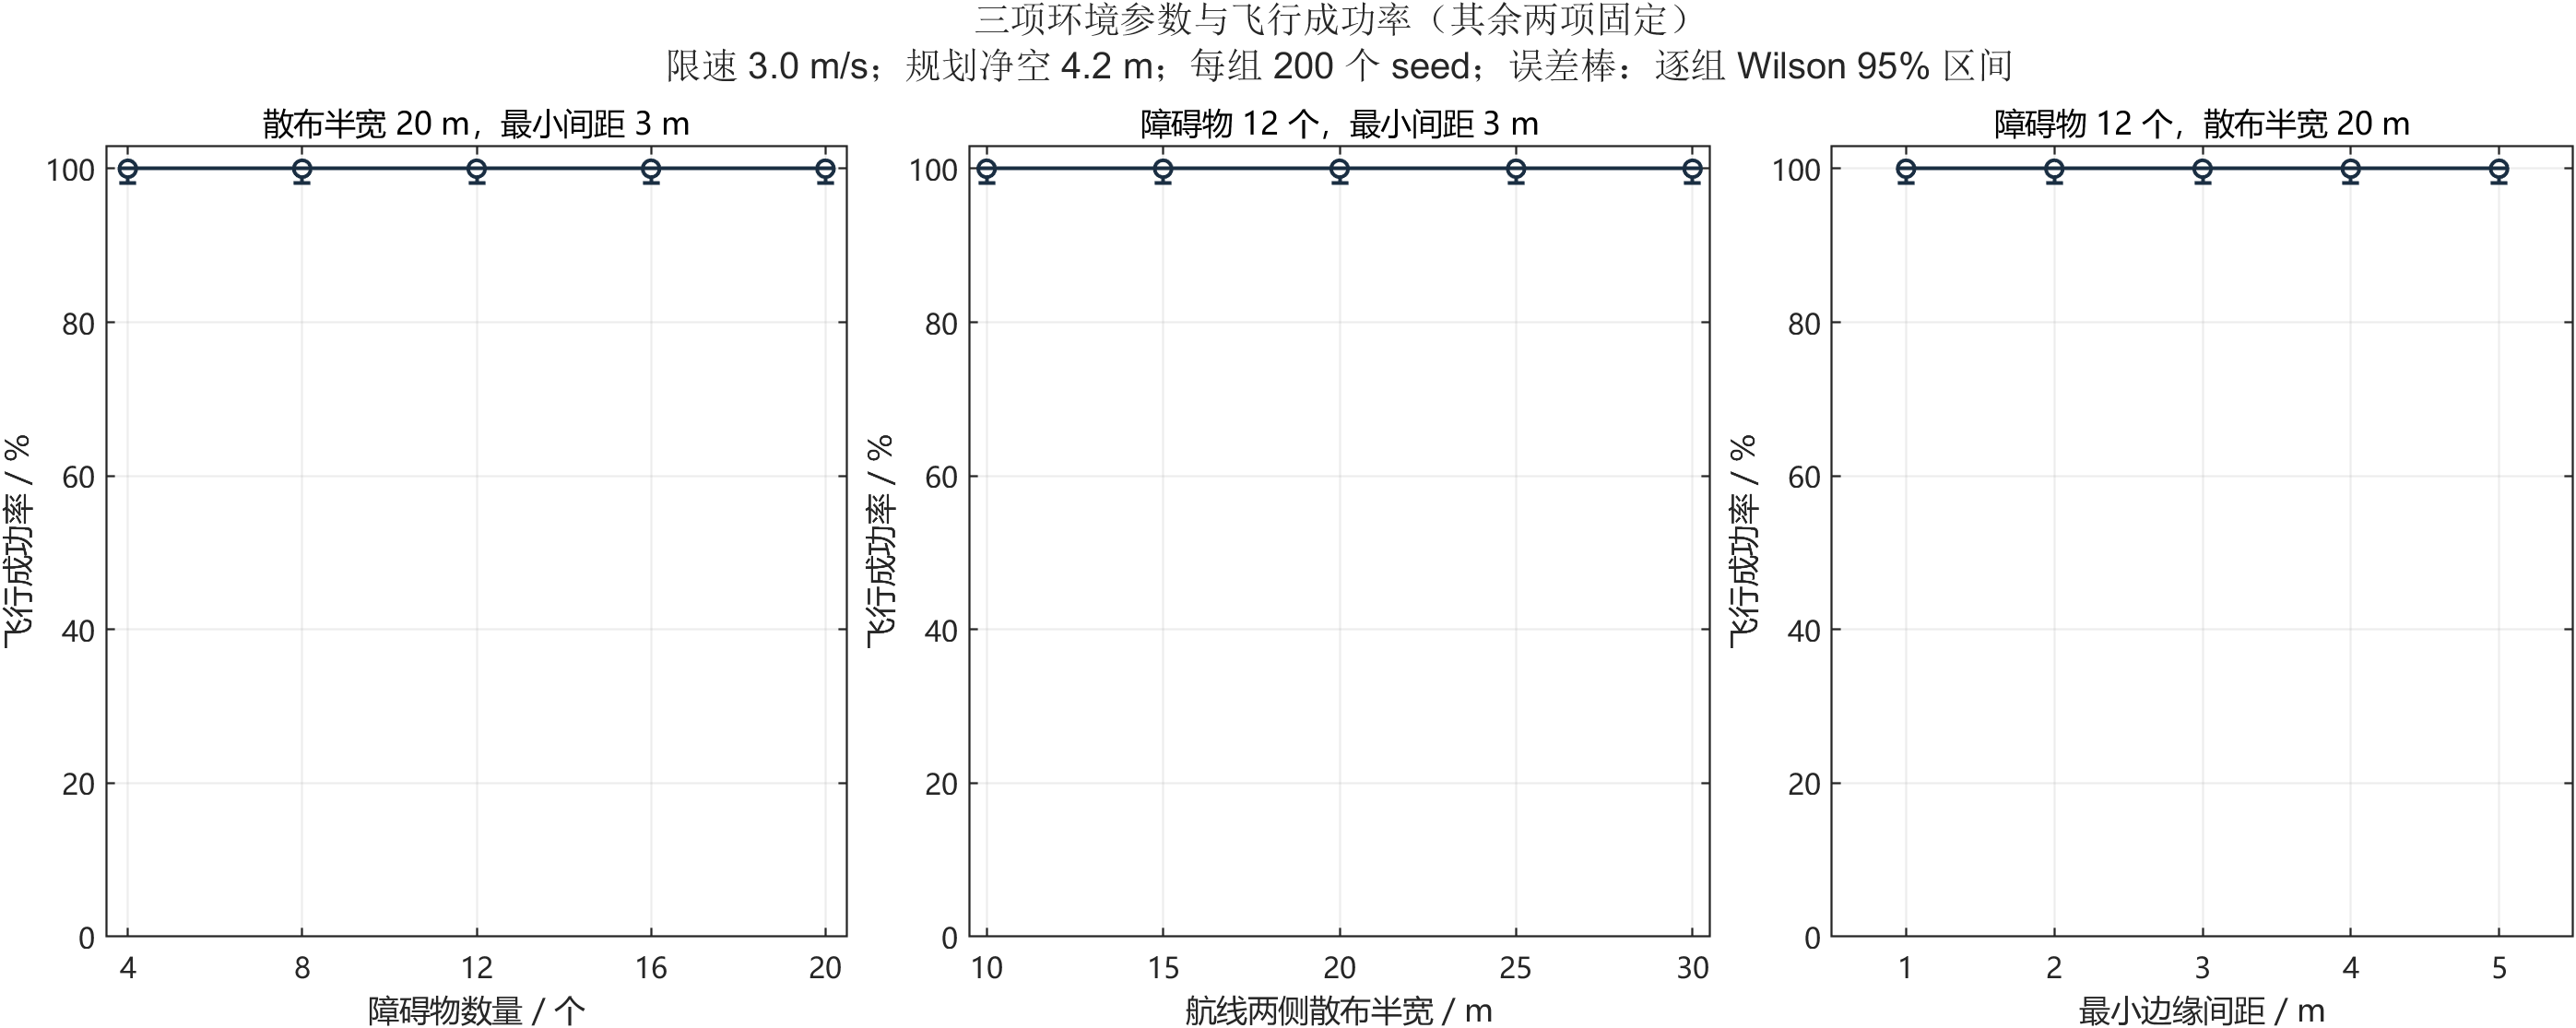
\includegraphics[width=0.98\textwidth]{01_factor_effects.png}
\caption{固定其余两项参数时的飞行成功率及逐组 Wilson 95\% 区间；每点最多 200 个已生成 seed。}
\label{fig:effects}
\end{figure}
\begin{figure}[H]\centering
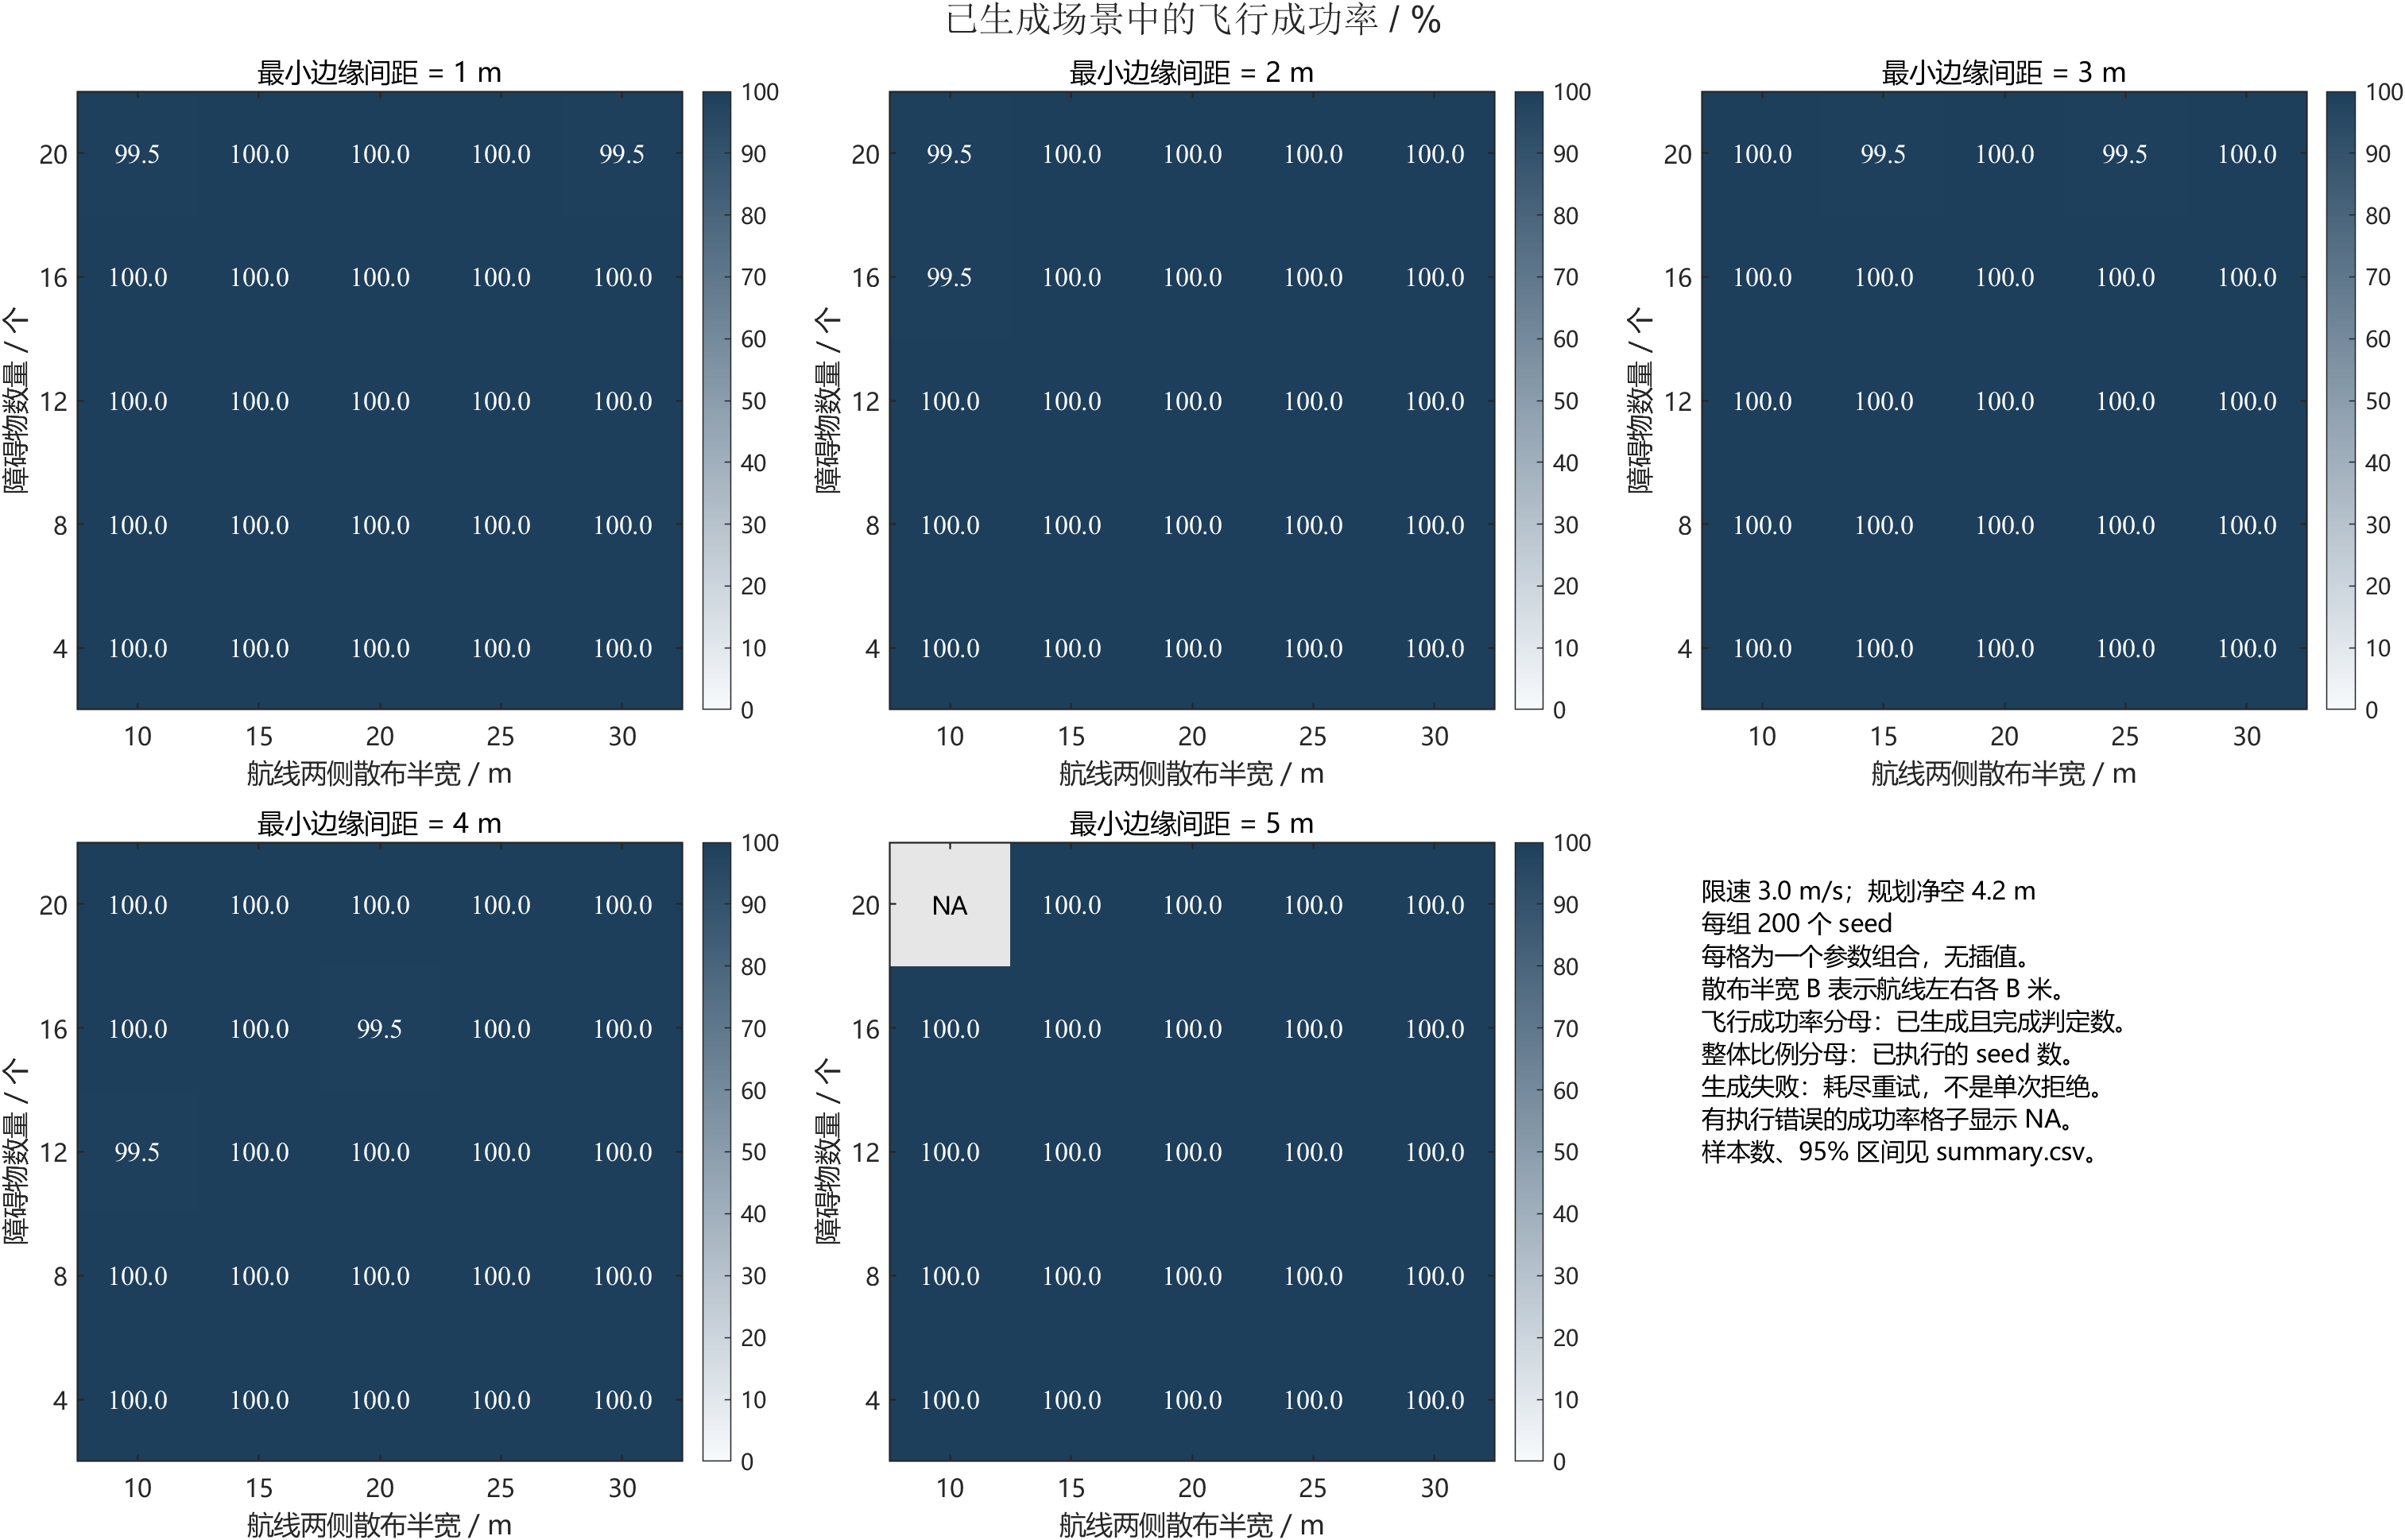
\includegraphics[width=0.98\textwidth]{02_flight_success_heatmaps.png}
\caption{125 组条件飞行成功率。若某格无已生成场景，则条件成功率无定义；不应解读为飞行失败。}
\label{fig:flight}
\end{figure}

生成失败集中在三个组合：$(M,B,g)=(20,10,4)$ 为 7/200，$(20,10,5)$ 为 200/200，$(20,25,5)$ 为 2/200，总计 209/25\,000。特别是 $(20,10,5)$ 在本次 seed 与生成器重试预算下没有生成一张可接受地图；图 \ref{fig:overall} 中该格的 0\% 是计划试验整体成功比例，\textbf{不是飞行成功率 0\%}。生成失败表示最多 60 次整组尝试、每个障碍最多 300 次放置尝试后仍未通过既定筛选，也不能证明该几何条件数学上无解。图 \ref{fig:genfail} 直接展示这类生成负担。

\begin{figure}[H]\centering
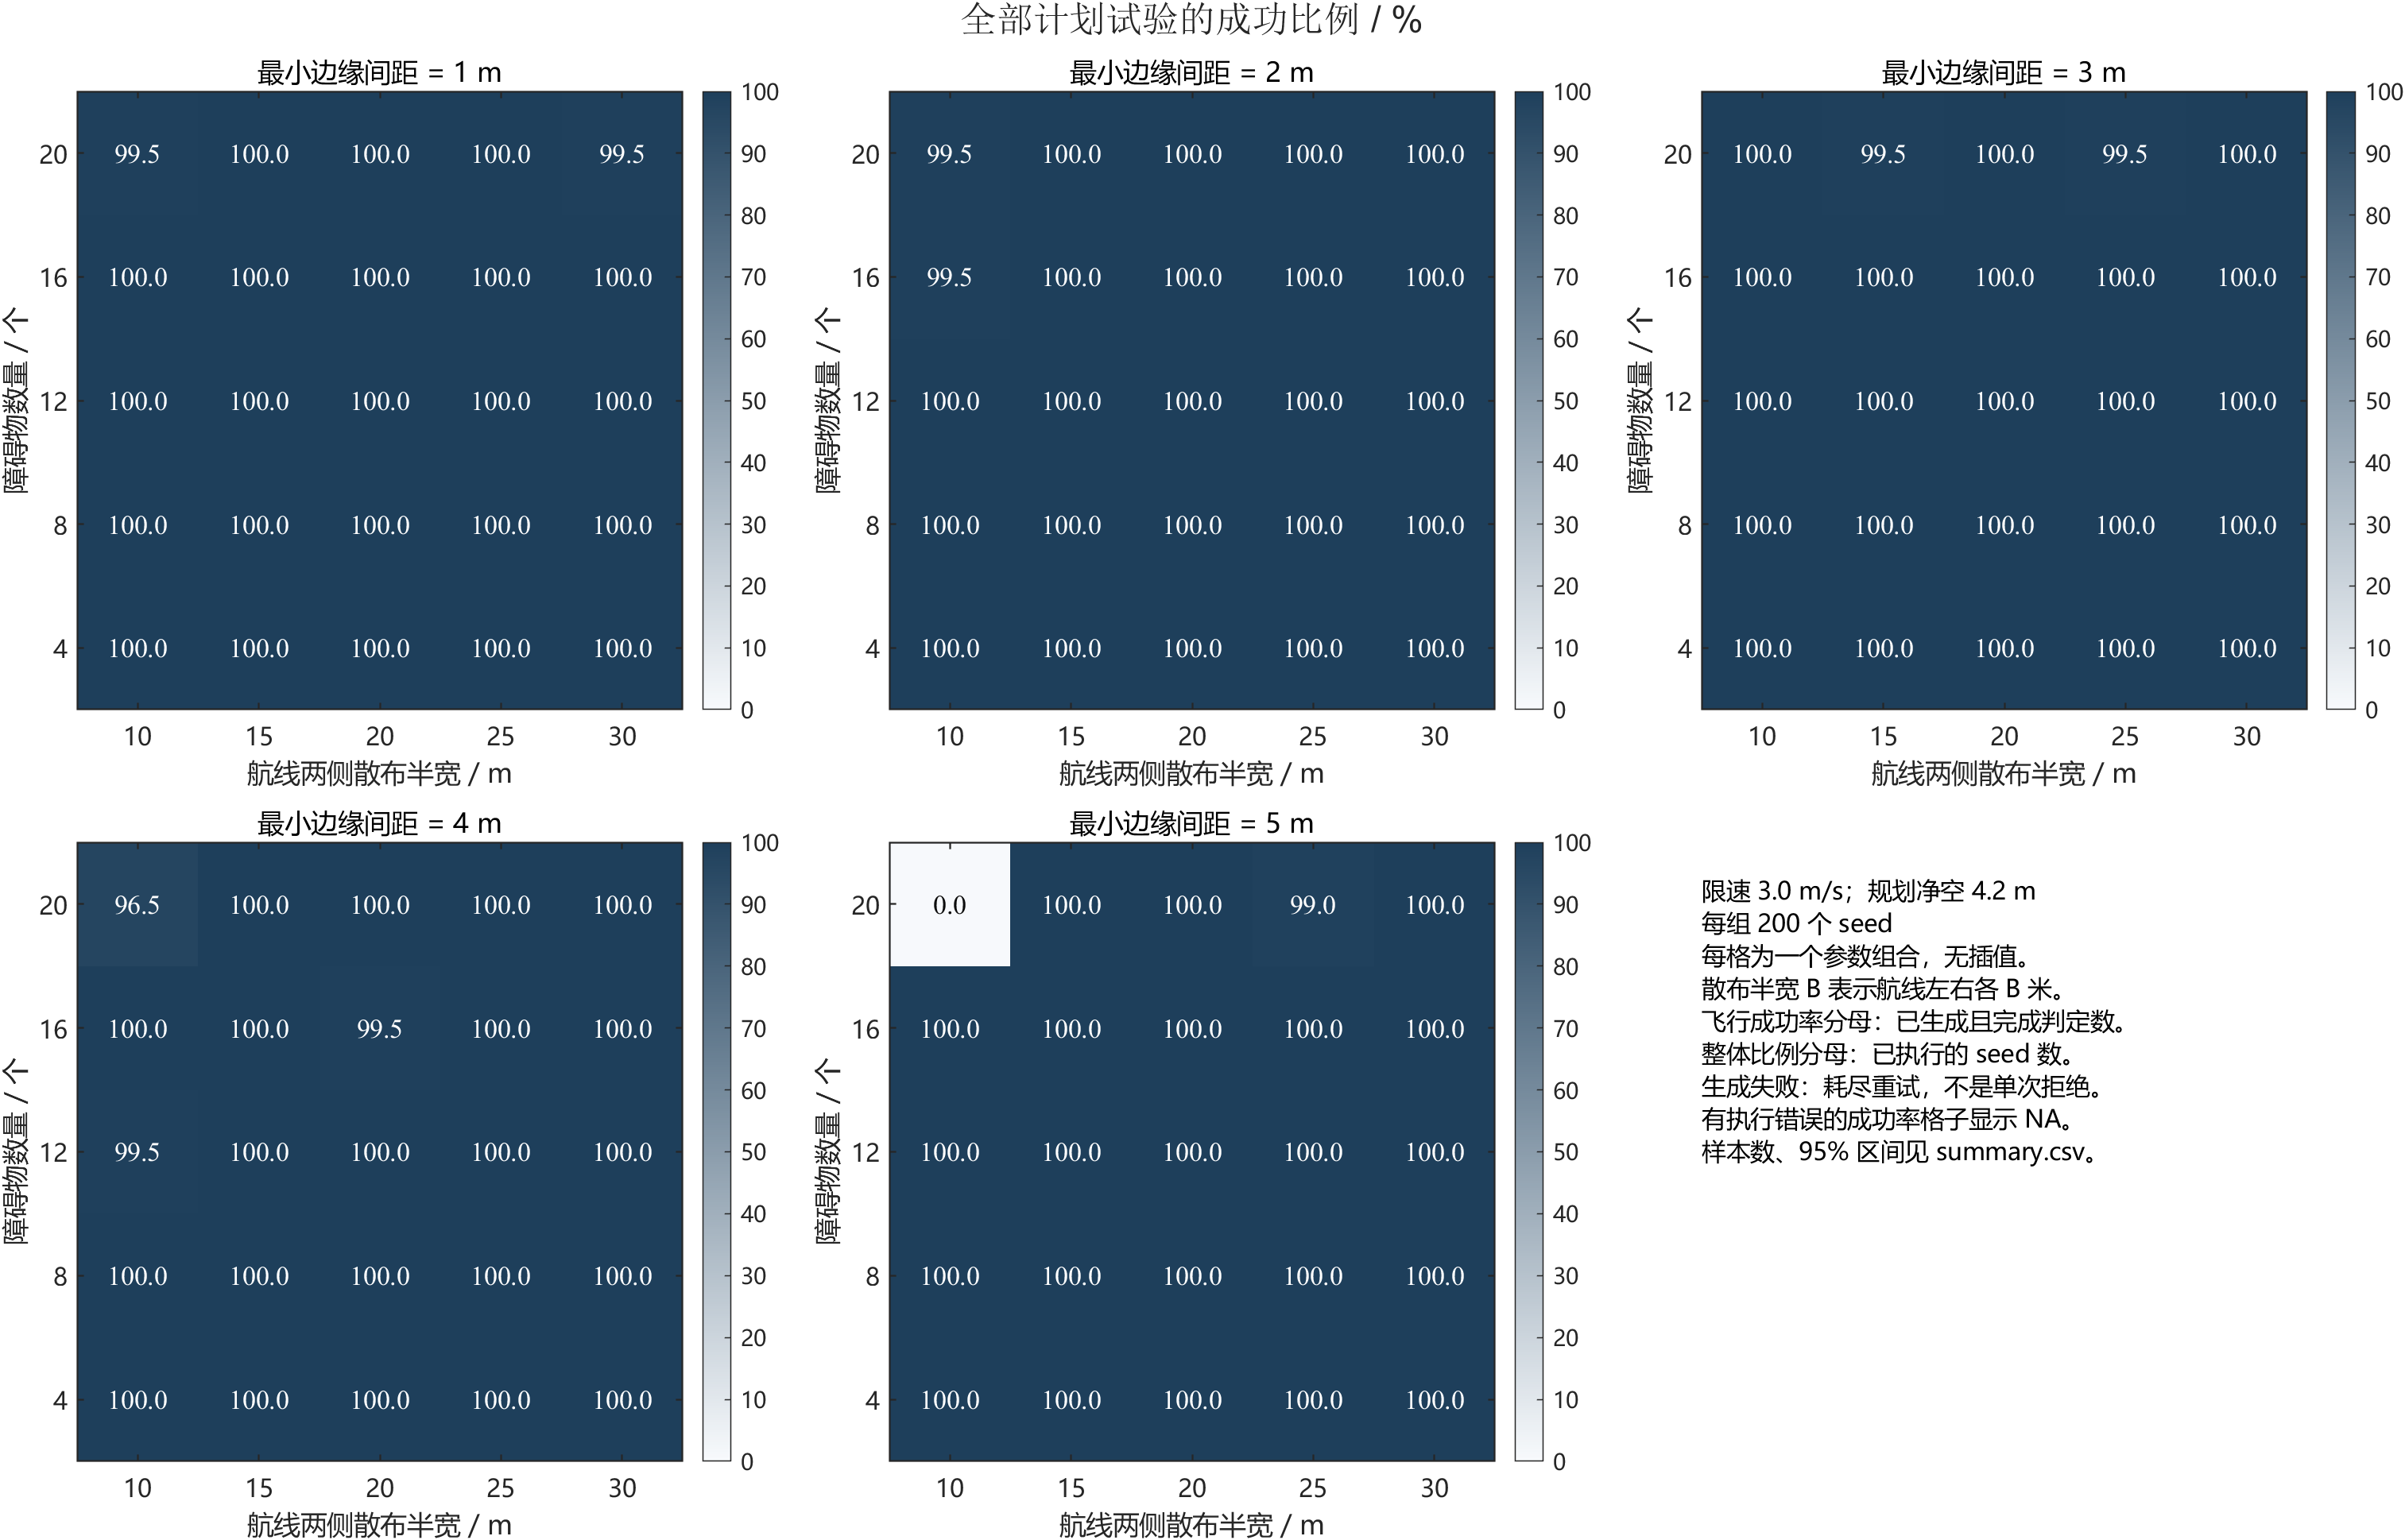
\includegraphics[width=0.98\textwidth]{03_overall_success_heatmaps.png}
\caption{全部计划任务的整体成功比例；分母包括场景生成失败。$(20,10,5)$ 的 0\% 来自 200/200 场景生成失败。}
\label{fig:overall}
\end{figure}
\begin{figure}[H]\centering
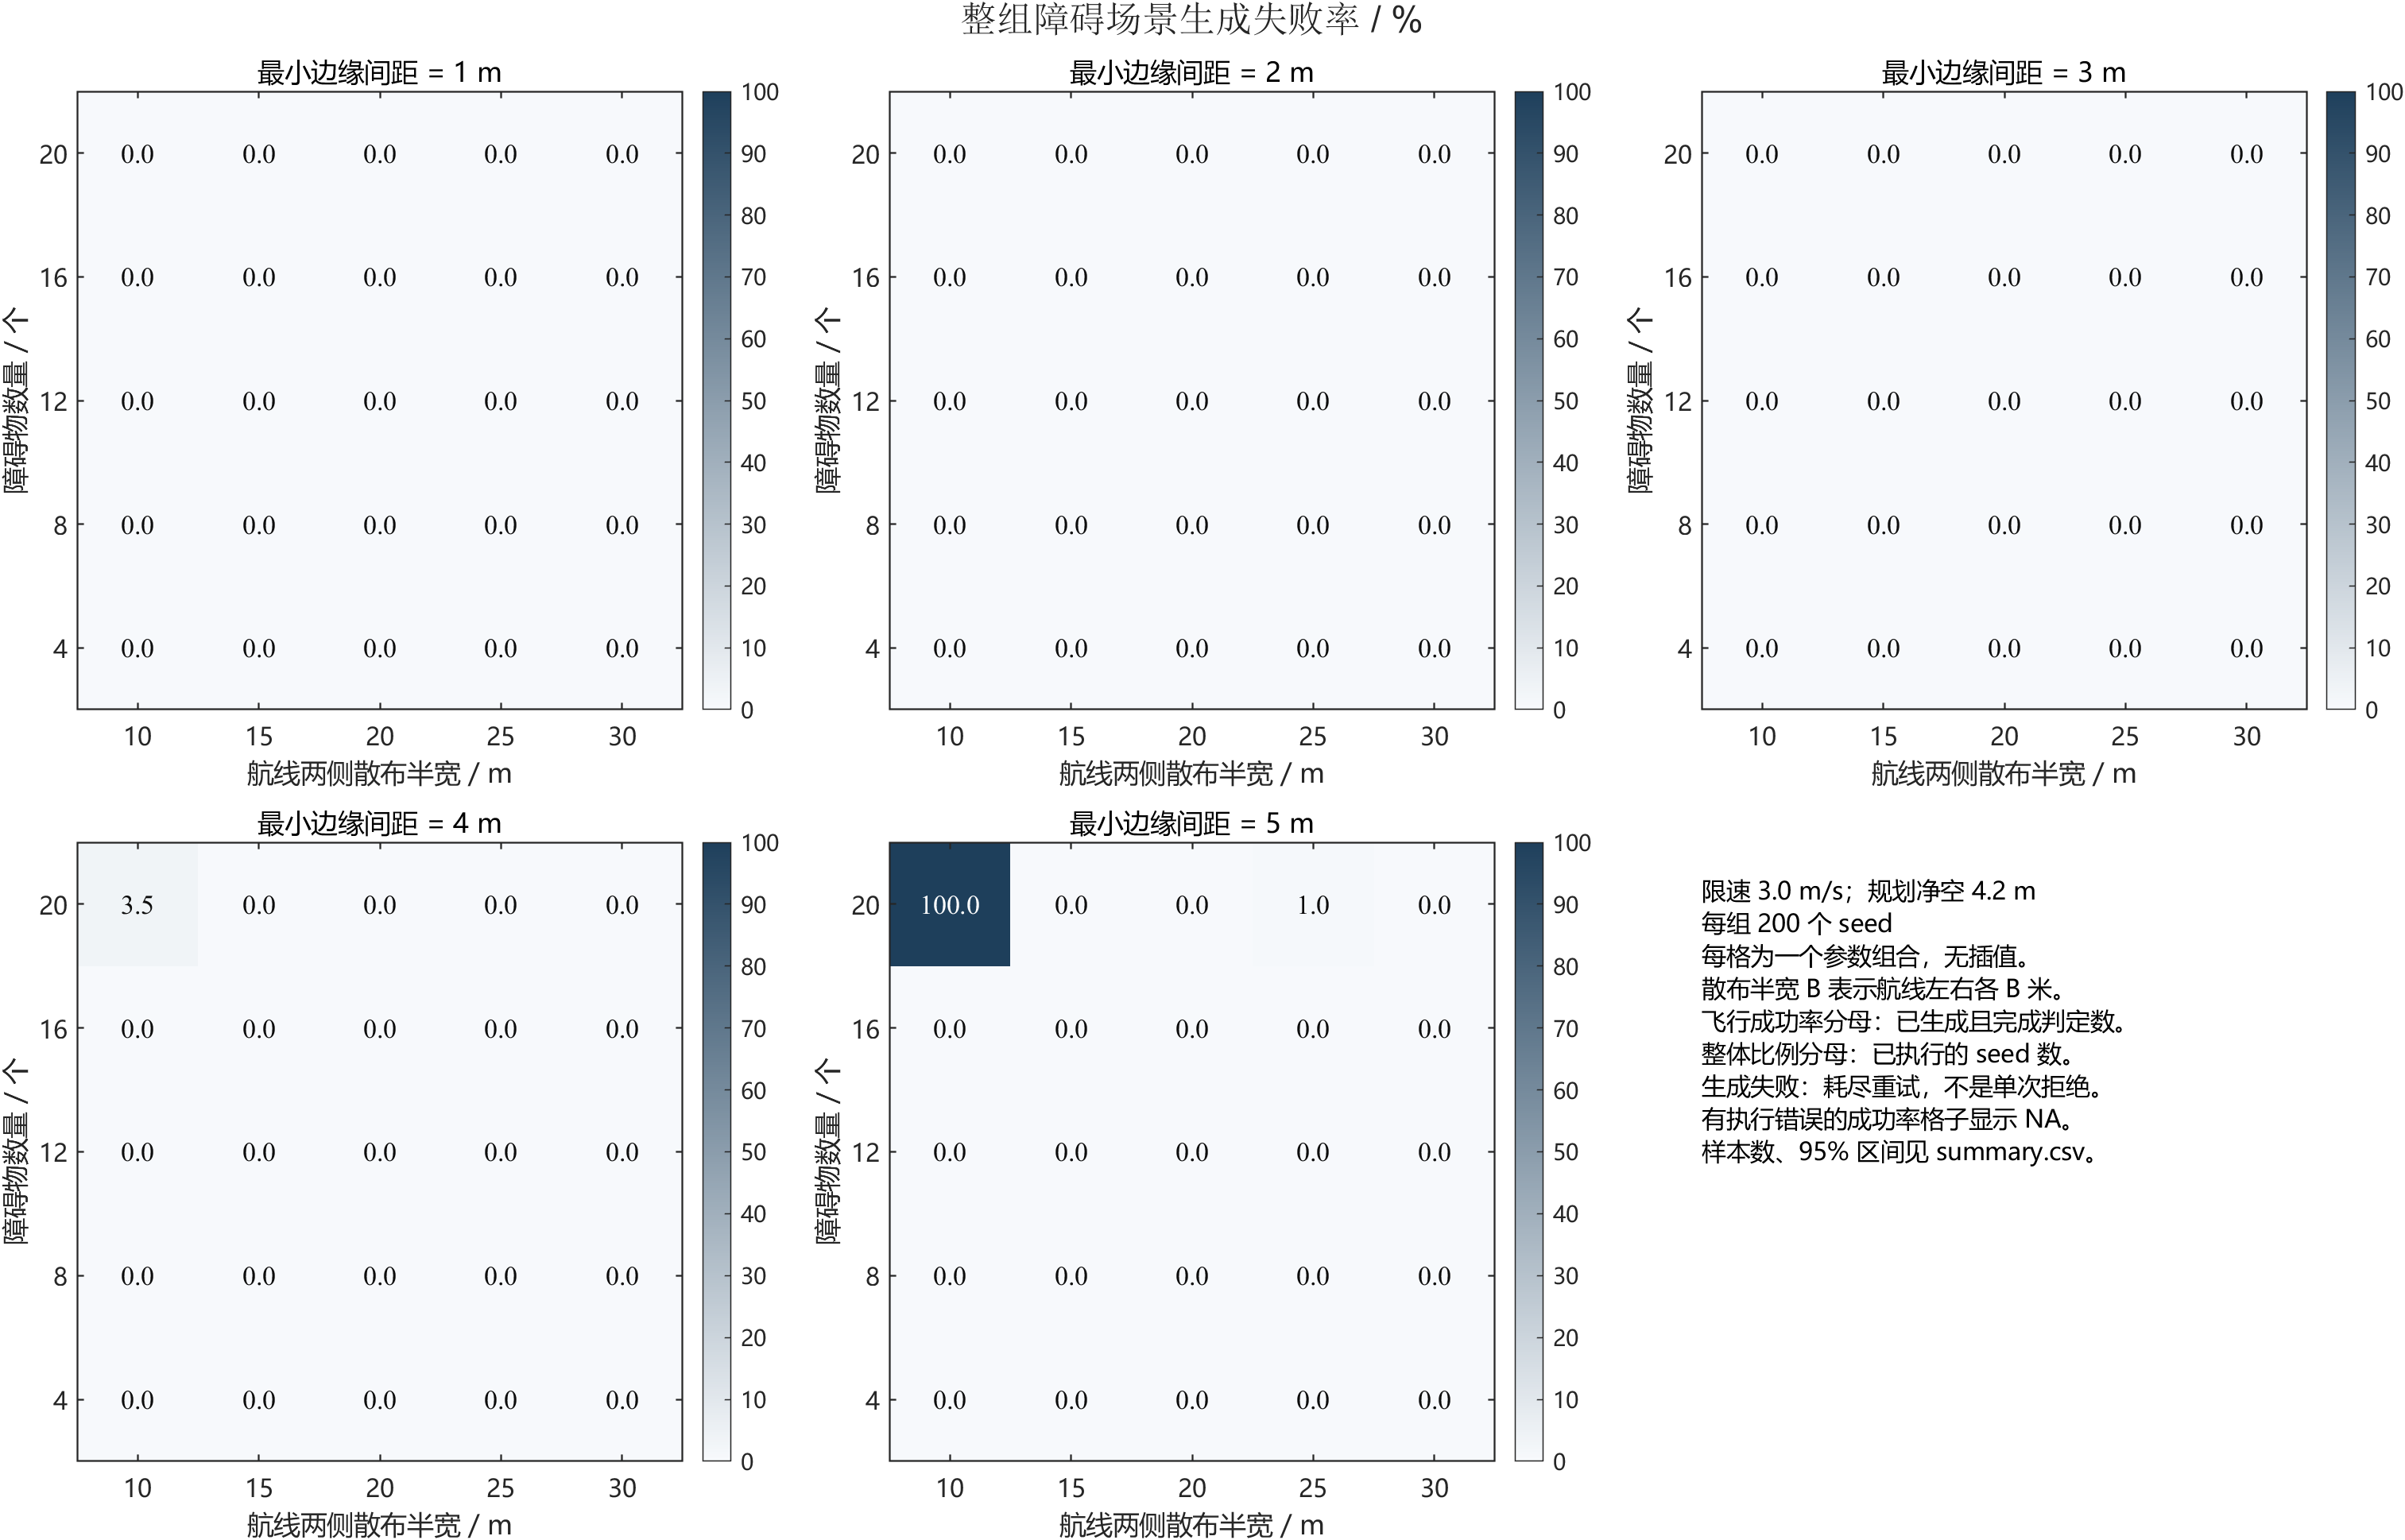
\includegraphics[width=0.98\textwidth]{04_generation_failure_heatmaps.png}
\caption{场景生成失败比例；它衡量当前生成器和筛选条件下的产出，不是飞行碰撞率。}
\label{fig:genfail}
\end{figure}

\subsection{完成时间、路径代价与队形误差}
对每个成功 seed 单独计算完成时间、长机路径系数和动态参考跟踪误差，再对该参数组合的成功样本取均值。图 \ref{fig:time} 展示完整网格的成功样本平均完成时间。为了避免三参数混杂，表 \ref{tab:center-count} 固定 $B=\SI{20}{m}$、$g=\SI{3}{m}$，只改变障碍物数量；五组各有 200/200 成功。
\begin{figure}[H]\centering
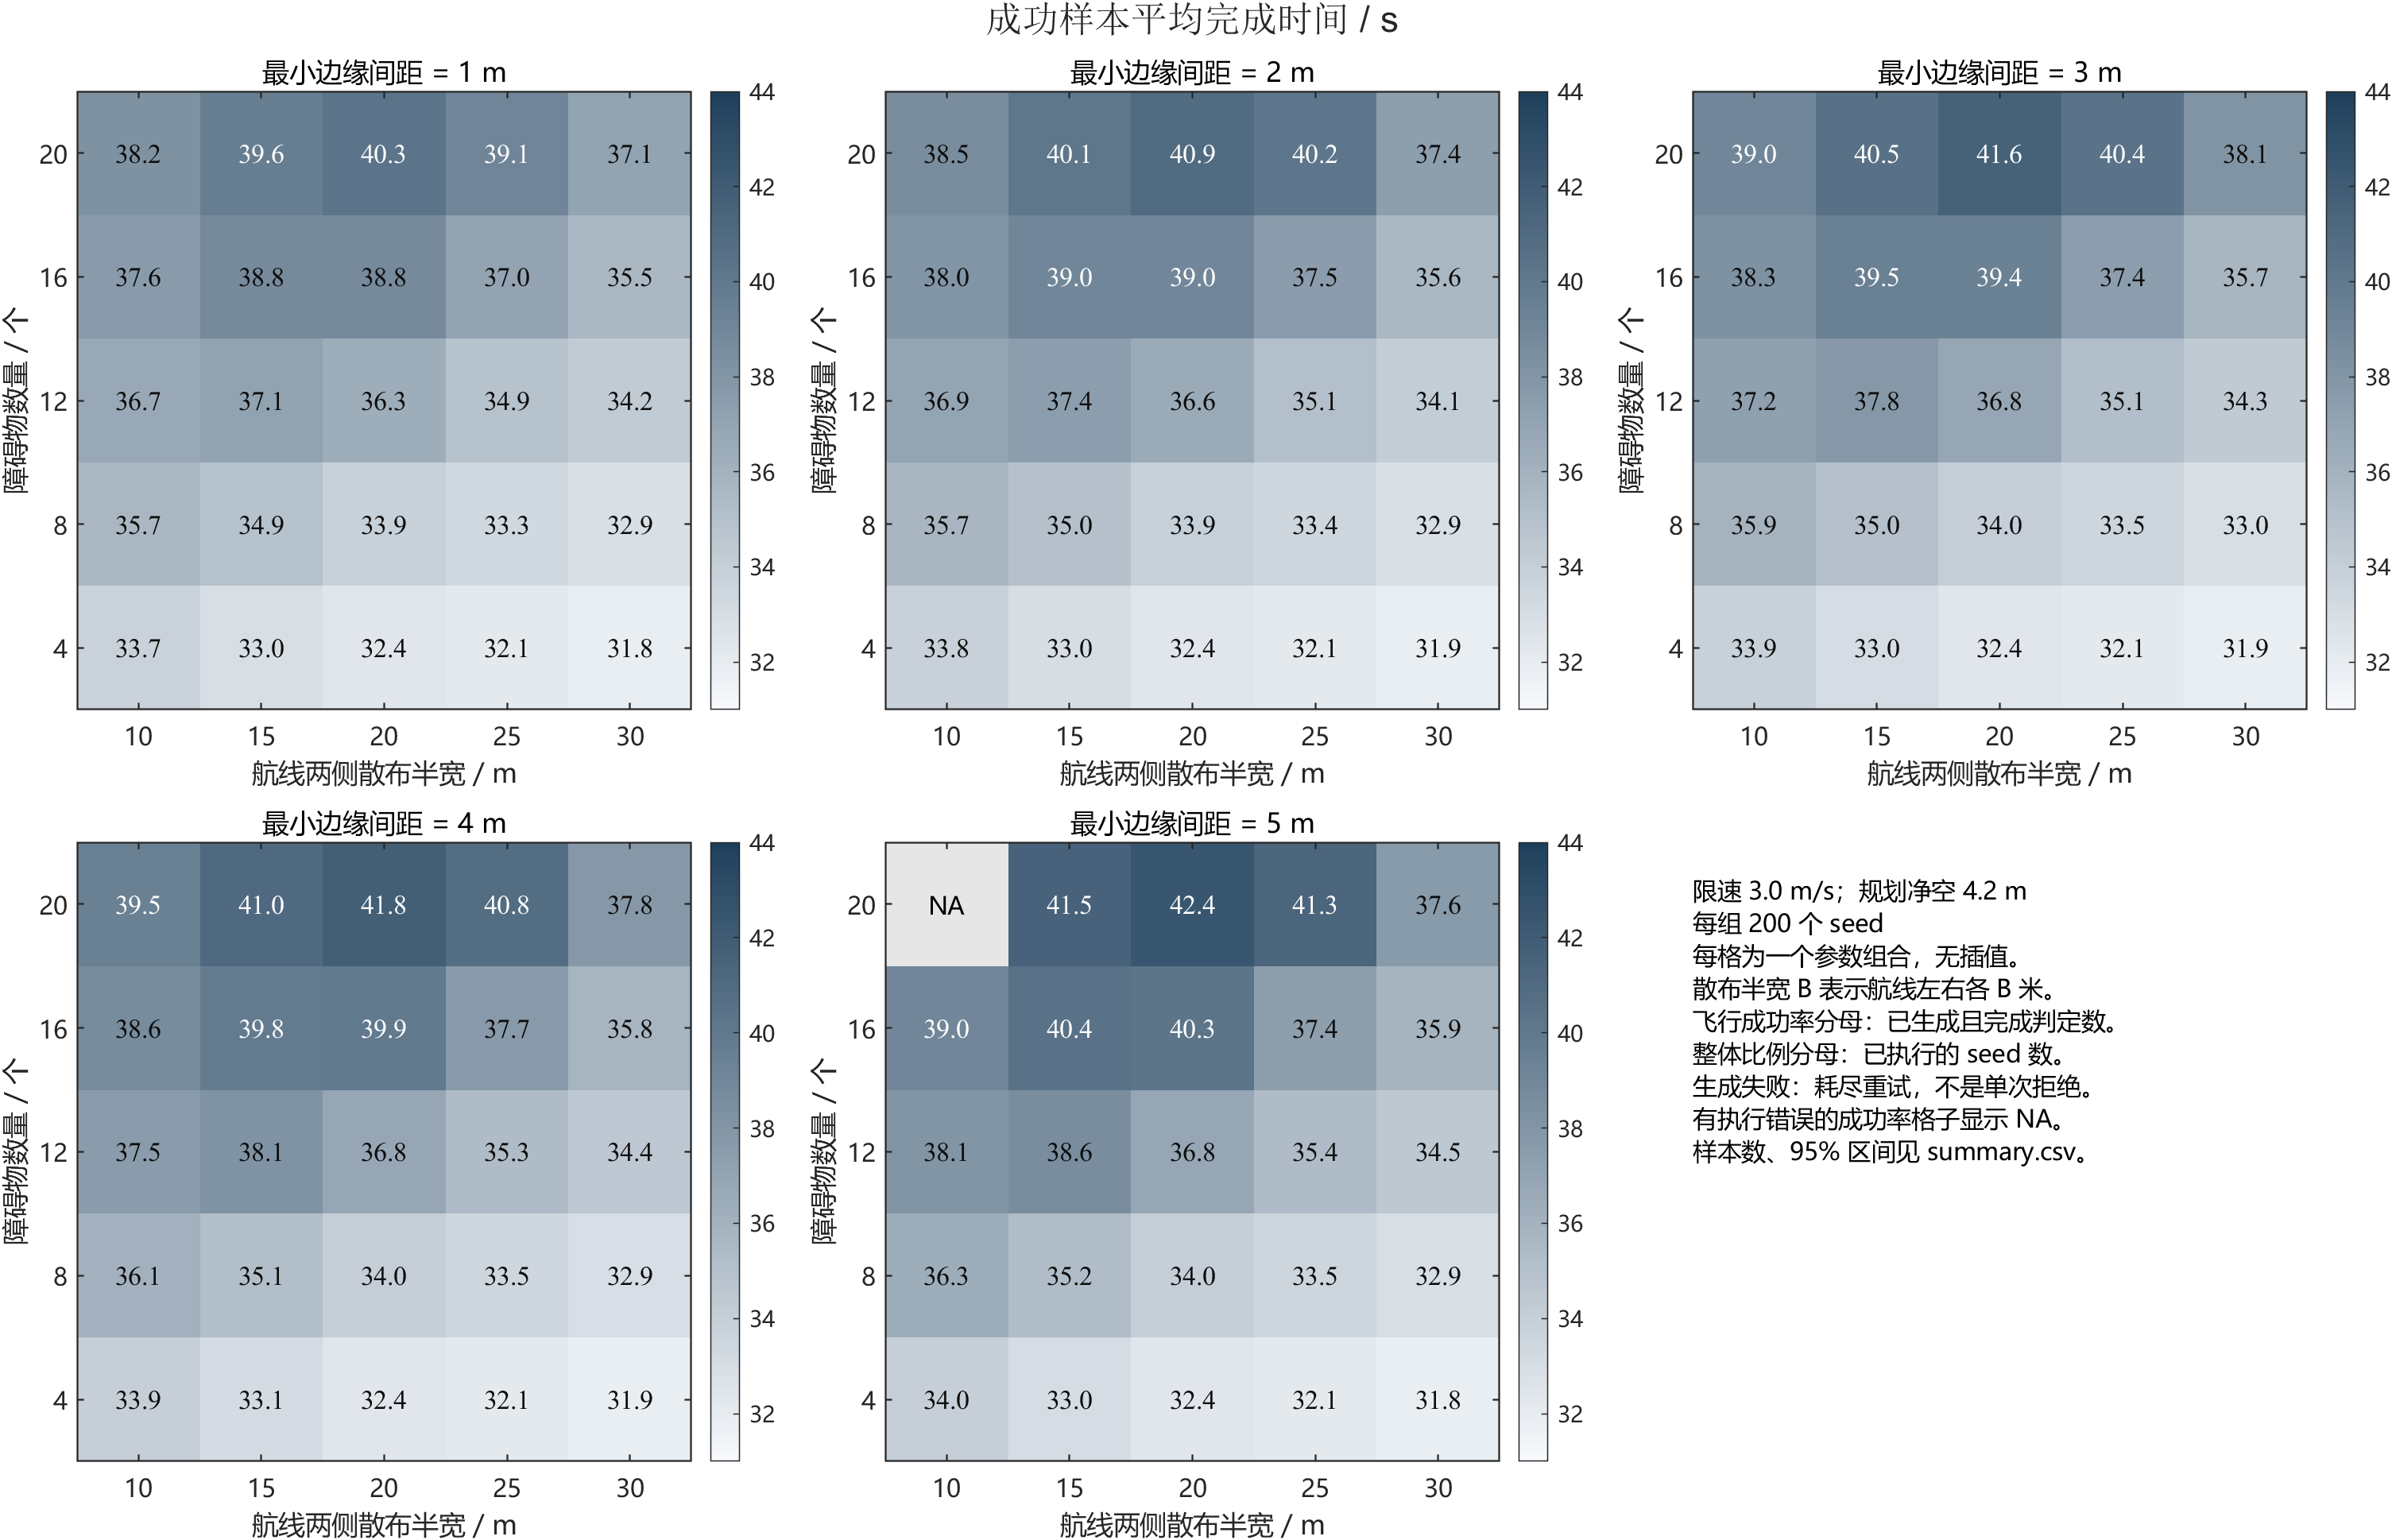
\includegraphics[width=0.98\textwidth]{05_completion_time_heatmaps.png}
\caption{各组合成功样本的平均任务完成时间，单位 s；没有成功样本的格子不应填入 0 s。}
\label{fig:time}
\end{figure}

\begin{table}[H]\centering\small
\caption{固定散布半宽 \SI{20}{m}、最小边缘间距 \SI{3}{m} 时的数量效应}
\label{tab:center-count}
\begin{tabular}{@{}rrrrr@{}}
\toprule
障碍物数 & 成功/已生成 & 平均时间/s & 长机平均路径系数 & 队形 RMS 均值/m \\
\midrule
4  & 200/200 & 32.37 & 1.036 & 3.46 \\
8  & 200/200 & 34.02 & 1.069 & 4.73 \\
12 & 200/200 & 36.84 & 1.147 & 5.95 \\
16 & 200/200 & 39.39 & 1.235 & 6.24 \\
20 & 200/200 & 41.57 & 1.309 & 6.60 \\
\bottomrule
\end{tabular}
\end{table}
在这条固定切片上，障碍物从 4 增至 20 个时，平均完成时间增加 \SI{9.20}{s}，长机路径系数增加约 0.272；动态参考队形 RMS 也上升。这是\textbf{该切片的观测关联}，不是所有宽度和间距下的单调定律。路径系数 1.309 表示长机成功轨迹平均约为直线距离的 1.309 倍，而不是多飞 130.9\%。

\begin{table}[H]\centering\small
\caption{固定另外两项参数时的完成时间切片；各格均 200/200 成功}
\label{tab:center-other}
\begin{tabular}{@{}rrrrrrrrrr@{}}
\toprule
\multicolumn{5}{c}{固定 $M=12,g=\SI{3}{m}$：散布半宽 $B$} &
\multicolumn{5}{c}{固定 $M=12,B=\SI{20}{m}$：边缘间距 $g$} \\
\cmidrule(lr){1-5}\cmidrule(l){6-10}
10 m & 15 m & 20 m & 25 m & 30 m & 1 m & 2 m & 3 m & 4 m & 5 m \\
\midrule
37.20 & 37.80 & 36.84 & 35.14 & 34.32 & 36.35 & 36.58 & 36.84 & 36.80 & 36.83 \\
\bottomrule
\end{tabular}
\end{table}
在固定 $M=12,g=\SI{3}{m}$ 的切片中，$B=\SI{30}{m}$ 的平均时间比 $B=\SI{10}{m}$ 低 \SI{2.87}{s}，但中间值并非严格单调。固定 $M=12,B=\SI{20}{m}$ 时，$g=1$--\SI{5}{m} 的时间仅落在 36.35--\SI{36.84}{s}，本轮数据不足以支持细微差异的稳定排序。散布采样超出场地时会被截断；在主扫描中，$B=30$ 的已生成场景有 41.46\% 至少出现一个被边界截断的障碍物，因此宽度增加不等于无偏地扩大开放空间。

\section{现行默认环境的独立补测}
\subsection{现行默认：16 个障碍、50 m 半宽、1 m 间距}
针对当前源码中主扫描未覆盖的默认设置，独立运行 seed 1--200，仍保持限速 \SI{3}{m/s} 与规划净空 \SI{4.2}{m}。结果 200/200 成功，0 次碰撞、0 次超时、0 次生成失败；逐组 Wilson 95\% 区间为 98.12\%--100\%。成功样本平均完成时间 \SI{33.45}{s}，长机平均路径 \SI{84.02}{m}、路径系数 1.058，动态参考队形 RMS 均值 \SI{4.15}{m}，最终最大队形误差均值 \SI{0.031}{m}。

该补测的 200/200 场景均至少有一个障碍物被工作空间边界截断。这意味着 \SI{50}{m} 是\textbf{采样前}的名义散布半宽，实际生成分布受到 \SI{80}{m}$\times$\SI{80}{m} 边界强烈影响。不能只凭该组较短完成时间断言把散布宽度继续增大就一定改善性能，也不能把 200/200 解释为系统的普遍安全保证。补测与主扫描分别保留独立的参数快照、逐 seed 数据和汇总表。

\section{闭环性质、超调与计算负担}
\subsection{局部稳定性能够证明到什么程度}
忽略障碍、机间作用、输入饱和及 ADP 在线更新，在非保持模式下固定参考位置时，僚机基础 PD 子系统可写为
\begin{equation}
\ddot{\bm e}+k_{\mathrm d}\dot{\bm e}+k_{\mathrm p}\bm e=\bm 0,\qquad
k_{\mathrm p}=2.6,\quad k_{\mathrm d}=1.8.
\end{equation}
其特征根为 $-0.9\pm1.338\mathrm j$，实部为负，故该\textbf{局部线性模型}渐近稳定；阻尼比约 0.558，标准二阶单位阶跃理论超调约 12.08\%，常用 2\% 调节时间近似为 \SI{4.44}{s}。长机固定目标保持模式的线性模型为 $\ddot{\bm e}_L+4\dot{\bm e}_L+6\bm e_L=\bm0$，特征根 $-2\pm1.414\mathrm j$，相应理论阶跃超调约 1.18\%、调节时间近似为 \SI{2.00}{s}。

僚机保持模式还会将增益提高到 $k_{\mathrm p}=3.9$、$k_{\mathrm d}=3.24$；在相同线性化假设下极点为 $-1.62\pm1.129\mathrm j$、标准阶跃理论超调约 1.10\%、近似 2\% 调节时间为 \SI{2.47}{s}。上述调节时间使用 $4/(\zeta\omega_n)$ 近似公式。

这些理论值不等于实际飞行轨迹的目标轴向超调：后者在本轮扫描中没有逐步轨迹数据可重算。完整系统还包含轨迹/模式切换、规划器、势场、限幅、非光滑安全修正与在线学习，以上线性极点不能推出完整闭环全局渐近稳定。25\,000 次计划试验只提供给定生成分布与参数上的经验性成功证据；8 次已生成地图的失败也表明不存在已证明的全场景收敛或零碰撞结论。

\subsection{算法规模}
记无人机数为 $N$、障碍物数为 $M$、栅格点数为 $G$、仿真步数为 $T$、安全层最多迭代次数为 $I$。现行 $N=5$、$G=81\times81=6561$、$T\leq10\,000$、$I\leq5$，主扫描 $M=4$--20。按实现结构，栅格占据计算为 $O(GM)$，稀疏八邻接图约有 $O(G)$ 条边；加权最短路搜索的常见实现量级为 $O((G+E)\log G)$。轨迹视线简化及起终点连接还会产生额外检查。每步 APF/机间处理约为 $O(NM+N^2)$，预测安全层最多放大到 $O(I(NM+N^2))$，状态与指标历史存储约为 $O(TN)$。此外，参考点的多轮障碍投影及回退候选搜索最坏约为 $O(NM^2)$，历史轨迹二分查找为 $O(N\log T)$；触发重规划的步还需承担路径规划成本。因此 $O(NM+N^2)$ 仅描述基础力计算，不是完整单步最坏复杂度。这是规模估计，不是对 MATLAB 内部图算法、重规划频率和生成器拒绝采样次数的精确运行时上界；高密度组合还可能把大量时间消耗在场景生成而非飞行仿真。

\section{结果解释、约束与下一步}
\begin{itemize}
\item \textbf{统计边界：}每组只有 200 个固定 seed。8 次飞行失败分散于 8 组，单格从 100\% 到 99.5\% 的差异不足以稳定排序。逐组 Wilson 区间不解决 125 组多重比较；从中挑选“最佳”环境或算法参数需要独立新 seed 验证。
\item \textbf{地图选择偏差：}场景生成先要求 \SI{5.6}{m} 整队通道；成功率仅适用于被该生成器接受的地图。209 次生成失败是生成器在有限重试预算下未产出，不是原始地图不可通行的概率，也不应计作飞行碰撞。
\item \textbf{空间参数解释：}最小障碍边缘间距 $g$ 是下限，非每图实际平均距离；增大散布半宽会触发工作空间边界截断。现行默认 $B=\SI{50}{m}$ 的 200 张地图全部发生至少一次截断，不能按无限平面的均匀散布来解释。
\item \textbf{队形含义：}巡航的动态参考跟踪误差可达数米，即使末端队形误差很小，也不能表述为“全航程紧密保持 V 形”。现行控制没有主动的障碍两侧分流--汇合决策。
\item \textbf{物理与证明范围：}模型为二维单位质量质点、静态圆障碍、全知地图和同步控制，未包含三维姿态、风扰、感知噪声、通信延迟、执行器动力学或动态障碍；预测避碰与 ADP 权重限幅不代替形式化安全或稳定性证明。
\end{itemize}
本轮最清晰的性能关联是：在固定 $B=\SI{20}{m},g=\SI{3}{m}$ 的切片上，障碍越多，完成时间、路径系数和动态队形误差均上升，而条件成功率仍处于统计天花板。若研究目标是比较环境难度对\textbf{飞行安全率}的影响，需要设计覆盖更难但仍可生成的地图，并扩大失败事件样本；若目标是改善编队形状，应在参考生成层研究弹性形变和分流--汇合，而不能只以终点归队误差评价飞行全过程。

\appendix
\section{数据来源与复现}
主扫描与默认环境补测分别于 2026 年 9 月 23 日和 24 日完成，权威记录保存在 F 盘项目的 results 目录。
两目录均有 \code{experiment.mat}、\code{trials.csv}、\code{summary.csv}
及源码快照；本报告同目录附逐 seed、分组统计及 SHA-256 CSV。
主扫描配置文件哈希以 \code{805c715a6971} 开头，完整值见附件。
本次从逐条记录独立核对：25\,000 个不同“组合--seed”键、125 组各
200 个 seed、各结局合计和组内均值均与汇总表一致；默认补测另有
200 个不同 seed，全部成功。主扫描可按 \code{docs/OBSTACLE\_SWEEP.md} 中的命令复现，且会新建结果目录。数据日期为 2026 年 9 月 23--24 日。本文均值从对应逐条记录汇总后按显示精度四舍五入，避免先对单次结果取整再平均；完整数值以CSV为准。报告附件分别保留两批实验的源码校验值；本次清单逐字节相同，表明两批使用同一冻结源码，但参数组合与结果仍分别统计。当前 \code{src/} 和 \code{config/} 的仿真核心源码与冻结快照逐字节一致；实验完成后只修正了扫描入口的任务备注和自动说明文字，不改变本次仿真数值。

\end{document}
